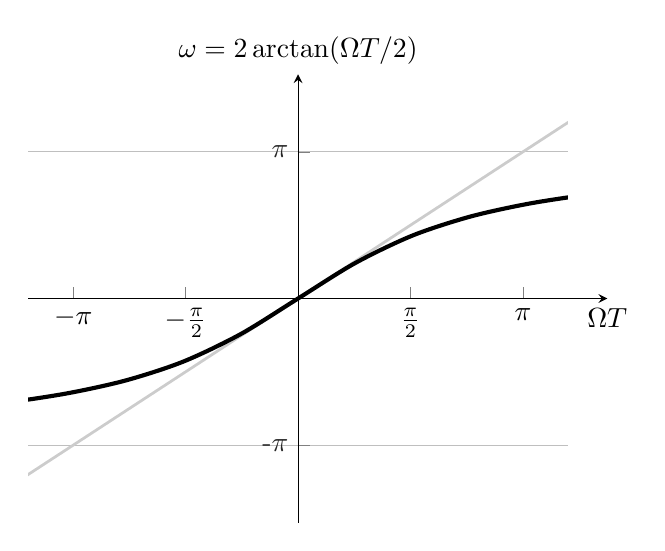
\begin{tikzpicture} 
\begin{axis}[
axis lines*=middle,
enlargelimits = true, clip=true,
xmax=3.14, xmin=-3.14,
ymin=-4, ymax=4,
y axis line style={->,>=stealth},
x axis line style={->,>=stealth, shorten >= -0.5cm},
xlabel={$\Omega T$},
ylabel={$\omega = 2\arctan(\Omega T/2)$},
every axis x label/.style={
    at={(ticklabel* cs:1)},
    anchor=north,
    xshift=0.5cm
},
every axis y label/.style={
    at={(ticklabel* cs:1)},
    anchor=south,
},
ytick={-3.14, 3.14}, yticklabels={-$\pi$, $\pi$},
xtick={-3.14, -1.57, 1.57, 3.14}, xticklabels={$-\pi$, $-\frac{\pi}{2}$, $\frac{\pi}{2}$, $\pi$},
%xmajorgrids,
ymajorgrids,
every outer y axis line/.append style={white!15!black},
every y tick label/.append style={font=\color{white!15!black}},
legend style={draw=white!15!black,fill=white,legend cell align=left}]

\addplot[smooth, black!20, solid, line width=1pt, domain=-20:20, samples=2] {x};
\addplot[smooth, black, solid, line width=1.5pt, domain=-20:20, samples=51] {rad(2*atan(x/2))};


\end{axis}
\end{tikzpicture}
